
\newpage
\newpage
\newpage
\pagebreak
\vspace{30cm}
\section{Aufgabe 1}
\textcolor{blue}{Erläutern Sie unter Verwendung geeigneter Hilfszeichnungen, wie viele Mikrofone grundsätzlich notwendig sind, um eine Schallquelle im Raum eindeutig zu lokalisieren. Gehen Sie dabei davon aus, dass Sie in der Lage sind mit einem Verfahren (das Sie später entwickeln werden), den Abstand zwischen der Schallquelle und jedem der Ihnen zur Verfügung stehenden Mikrofone zu bestimmen.\\ Ihre Erläuterung muss nachvollziehbar sein. Gehen Sie dabei schrittweise vor. Diskutieren Sie den Fall, dass nur ein Mikrofon zur Verfügung steht und erklären und belegen Sie, weshalb ein Mikrofon vermutlich nicht ausreichend ist. Dann erhöhen Sie schrittweise die Anzahl der Mikrofone solange, bis Sie eindeutig den Ort der Schallquelle bestimmen können. } 
\subsection{Anzahl der benötigten Mikrofonzahl}
\subsubsection{Auswertung mit einem Mikrofonen}
Ein Mikrofon könnte nur den Abstand \textit{r} der Schallquelle zum Mikrofon erkennen. Diese Annahme beruht auf dem Text der Aufgabenstellung. Damit ist keine Positionserkennung möglich, da alle Punkte mit Abstand \textit{r} infrage kommen. 
Alle diese möglichen Punkte bilden eine Kugeloberfläche um den Mittelpunkt (die Position des Mikrofons), mit dem Abstand \textit{r}.

\subsubsection{Auswertung mit zwei Mikrofonen}
Mit zwei Mikrofonen ist eine Eingrenzung der möglichen Positionen der Schall-quelle möglich, da nur noch die Schnittmenge der beiden Kugeloberflächen um die Mikrofone als Positionen in Frage kommen. Diese Schnittmenge stellt einen zweidimensionalen Kreisumfang dar. Siehe Abbildung \ref{fig:Normalfall beim Schnitt zweier Kugeloberflächen}. Dieser besteht aber immer noch aus $\infty$ Punkten und ist deshalb im Normalfall nicht geeignet zur Positionsbestimmung. Nur für den Sonderfall, dass die Schallquelle exakt im Mittelpunkt der Geraden zwischen Mikrofon 1 und 2 liegt kann die Position eindeutig bestimmt werden. Siehe Abbildung \ref{fig:Sonderfall beim Schnitt zweier Kugeloberflächen}.
\begin{figure}[b]
	\centering
	\begin{minipage}[t]{0.45\linewidth}
		\centering
		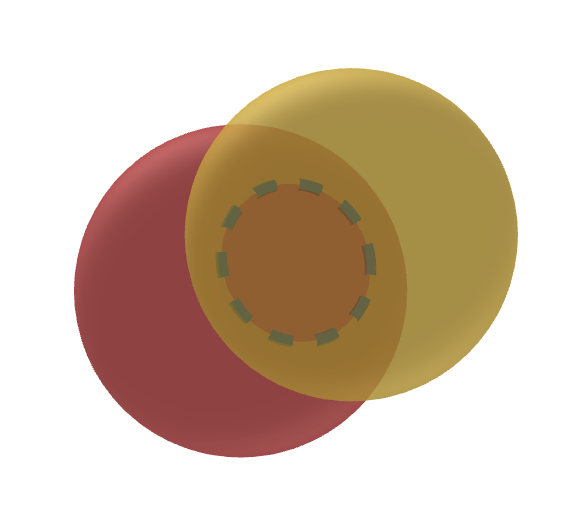
\includegraphics[width=0.75\textwidth]{Schnitt_2_Kugeln}
		\caption{Normalfall beim Schnitt zweier Kugeloberflächen}\label{fig:Normalfall beim Schnitt zweier Kugeloberflächen}		
	\end{minipage}
	\hfill
	\begin{minipage}[t]{0.45\linewidth}
		\centering
		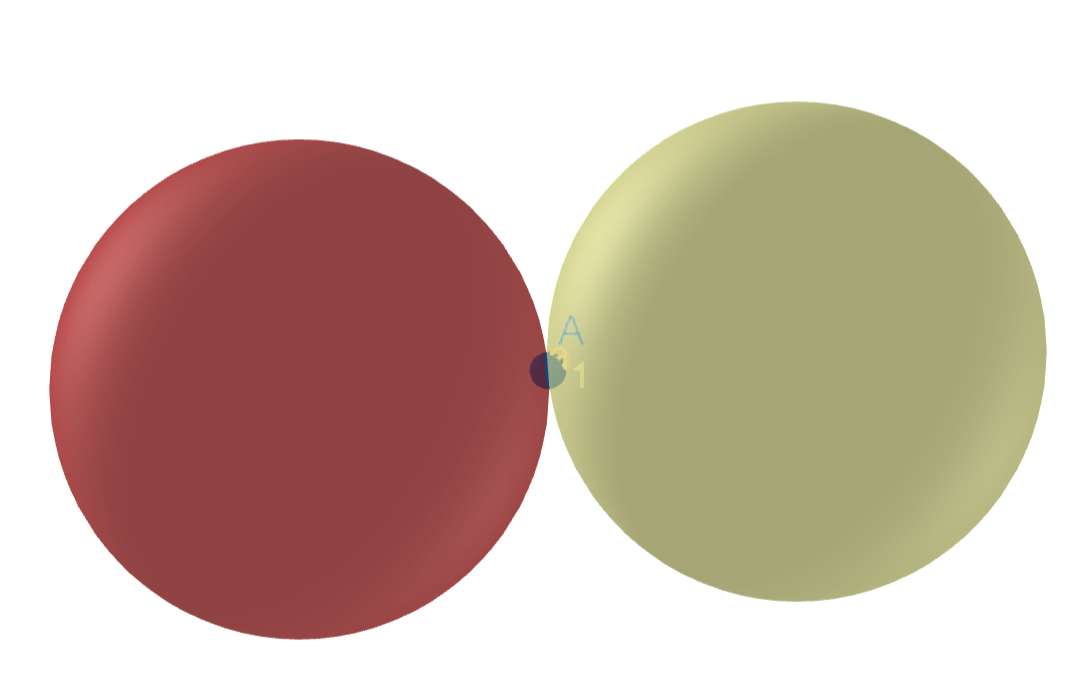
\includegraphics[width=0.75\textwidth]{2KugelnSonderfall}
		\caption{Sonderfall beim Schnitt zweier Kugeloberflächen}\label{fig:Sonderfall beim Schnitt zweier Kugeloberflächen}
	\end{minipage}
\end{figure}

\subsubsection{Auswertung mit drei Mikrofonen}

Durch die Detektion der Schallquelle mit drei Mikrofonen ist die Eingrenzung der möglichen Orte der Schallquelle auf zwei Punkte möglich. Die Orte der drei Schallquellen bilden immer eine Ebene im Raum, es ist nicht möglich, dass sich nur zwei in einer Ebene befinden und das Dritte außerhalb liegt. Darin liegt auch das Problem der zwei Punkte. Einer der beiden Punkte liegt oberhalb der Ebene aus den Mikrofonen mit einem Abstand $\lambda$ zur Ebene. Der Zweite liegt auf einer Geraden, die durch den ersten möglichen Punkt verläuft und orthogonal zur Mikrofonebene ist. Er hat den Abstand -$\lambda$ zur Ebene. Siehe Abbildung \ref{fig:Schnittpunkte dreier Kugeloberflächen}. \\
Bei der Aufgabenstellung soll ein Raum mit\\ 1m x 1m x 1m Größe nach der Schallquelle durchsucht werden. Wenn die Mikrofonebene in einer der Begrenzungsebenen des Versuchsraums liegt, reichen 3 Mikrofone aus, da der andere Schnittpunkt der möglichen Orte der Schallquelle damit außerhalb des Versuchsraums liegt.\\ Wenn die Mikrofonebene keine der Raumbegrenzungsebenen darstellt, sind drei Mikrofone nicht ausreichend. 
\begin{figure}
\centering 
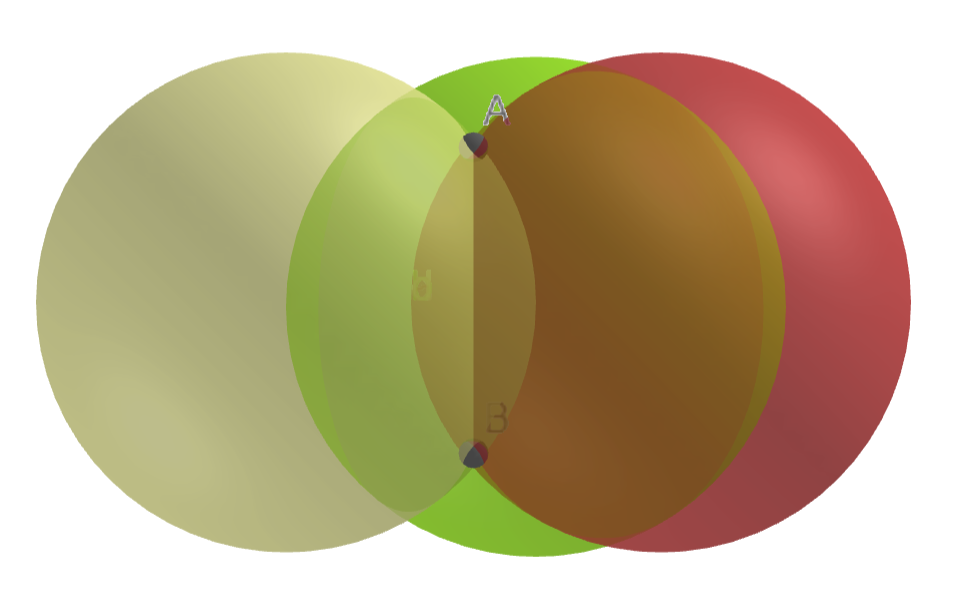
\includegraphics[width=0.4\textwidth]{3Kugeln}
\caption{Schnittpunkte dreier Kugeloberflächen}\label{fig:Schnittpunkte dreier Kugeloberflächen}
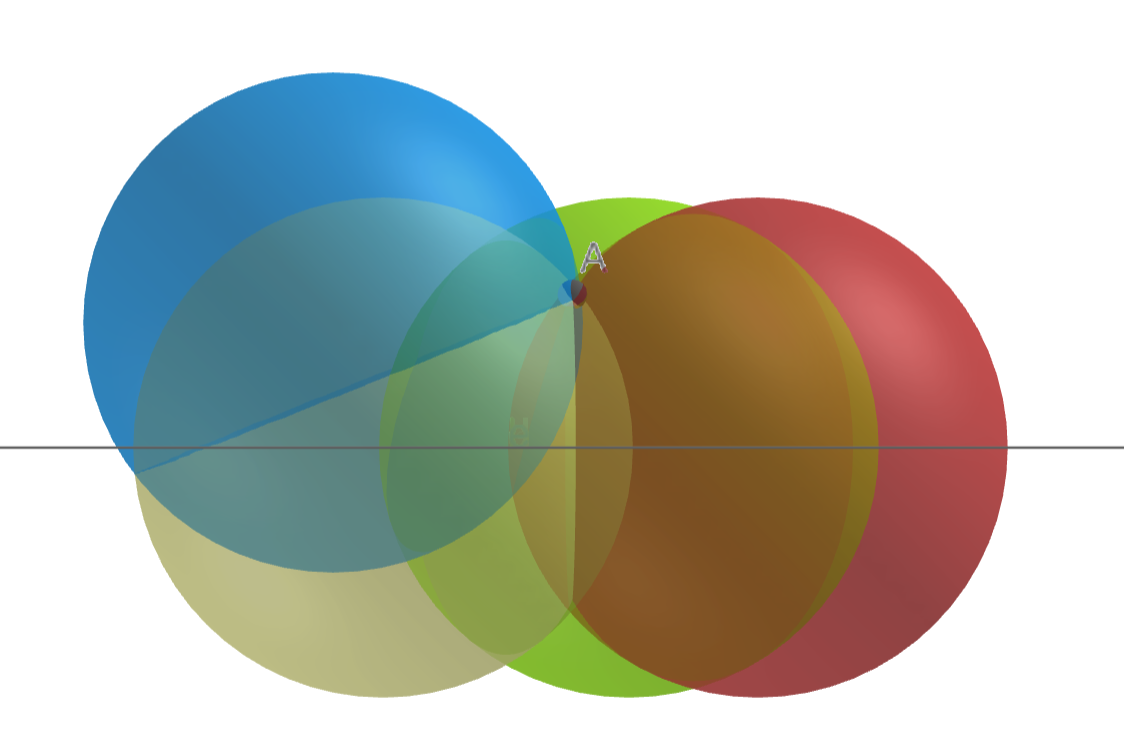
\includegraphics[width=0.4\textwidth]{4Kugeln}
\caption{Eindeutige Schnittpunktbestimmung durch vier Kugeloberflächen}\label{fig:Eindeutige Schnittpunktbestimmung durch vier Kugeloberflächen}
\end{figure}
\subsubsection{Auswertung mit 4 Mikrofonen}
In unserem Fall haben wir nicht die absolute Distanz, zwischen Schallquelle und Mikrofon, sondern nur die Laufzeitunterschiede zwischen den einzelnen Mikrofonen.Und somit die Distanzunterschiede zur Schallquelle. Im dreidimensionalen Raum benötigen wir drei Informationen. Um drei Laufzeitdifferenzen zu erhalten, benötigen wir vier Mikrofone. 

Wenn sich das vierte Mikrofon nicht in einer Ebene mit den anderen dreien befindet, kann dadurch die Eindeutigkeit des Schnittpunktes zeitgleich garantiert werden. Da damit einer der beiden Schnittpunkte aus dem Fall mit drei Mikrofonen wegfällt. Siehe Abbildung \ref{fig:Eindeutige Schnittpunktbestimmung durch vier Kugeloberflächen}. Für unser Newtonverfahren müssen wir also mit vier Mikrofonen den Versuch aufbauen.



%______________________________________________________________________________________________
\newpage
\pagebreak
\section{Aufgabe 2}
\textcolor{blue}{Nachdem Sie nun wissen, wie viele Mikrofone Sie benötigen, untersuchen Sie die Genauigkeit der Methode. Martin Bossert beschreibt im Buch "Mathematik der digitalen Medien: präzise, verständlich, einleuchtend", ein Verfahren, das iterativ den Ort bestimmt, wenn die Wege(unterschiede) des Schalls zu den einzelnen Mikrofonen bekannt sind. Auszüge aus dem Buch finden Sie auf Relax. 
Gehen Sie dabei davon aus, dass Sie eine Schallquelle in einem Quader mit den Abmessungen 1 x 1 x 1 m bestimmen wollen.  Implementieren Sie das Verfahren von Bossert in Matlab und simulieren Sie verschiedene Szenarien (z.B. Mikrofone an den Ecken des betrachteten Raums, d.h. große Distanz der Mikrofone oder eine Konstellation, bei der die Mikrofone nur wenige cm voneinander entfernt sind). Gehen Sie nun davon aus, dass Sie über eine Methode verfügen, die den Abstand zur Schallquelle mit einer Genauigkeit von $\pm$ $\varepsilon$ bestimmen kann. Wie wirkt sich diese Ungenauigkeit auf die Ortsbestimmung aus und welche Konstellation der Mikrofone liefert hierfür die besten Ergebnisse? Wie sollten Sie die Mikrofone bestmöglich anordnen?  Möglichst weit auseinander an den Ecken des Quaders oder kompakt und relativ nah zusammen? \\
Stellen Sie die Ergebnisse anschaulich und übersichtlich dar. Sie haben viele Freiheitsgrade, d.h. Sie können viele Ergebnisse produzieren. Die Schwierigkeit besteht darin, die Vielzahl der möglichen Ergebnisse zusammenzufassen und in aussagekräftigen Diagrammen darzustellen. \\
Ein Beispiel, wie Sie Ergebnisse effizient darstellen können: Sie schreiben ein Programm, das die Schätzung bei einer gegebenen Mikrofon-Konstellation für eine Vielzahl von Orten der Schallquelle simuliert. Sie speichern die Simulationsergebnisse (z.B. den Schätzfehler in Abhängigkeit von tatsächlichem Ort und der Konstellation der Mikrofone) und erzeugen dann Charts, die beispielsweise den Schätzfehler (absolut oder relativ) in Abhängigkeit von der tatsächlichen Distanz zu den Mikrofonen darstellen. Wenn sich dabei Zusammenhänge zeigen, dann ist dieser Graph geeignet um die Ergebnisse darzustellen. Wichtig ist, dass Sie das Diagramm nicht nur zeigen, sondern auch beschreiben und Daraus Rückschlüsse/Schlussfolgerungen ziehen.}
\subsection{Mathematischer Ansatz: Newtonverfahren}
Aus den Zeitverschiebungen, mit der das Signal der Schall-quelle von den Mikrofonen aufgenommen wird, kann die Position der Schallquelle im Raum näherungsweise bestimmt werden. Für das Newtonverfahren muss ein erster Ort der Schallquelle geschätzt werden, von welchem aus in mehreren Iterationen der reale Ort der Schallquelle immer besser angenähert werden kann. In einigen Fällen kommt das Newtonverfahren aber zu keinem korrekten Ergebnis. Das ist abhängig von der Positionierung der Mikrofone im Raum, dem Ort der Schallquelle, sowie der Schätzung der ersten Position des Objekts. 

Die Zeitverschiebung der Signale kann durch die Korrelation der Signale S1, S2 und S3 gegen das Signal S0 berechnet werden. Im Buch "Mathematik der digitalen Medien" von Bossert und Bossert wird das Verfahren für den zweidimensionalen Raum sehr ausführlich beschrieben. Weitere Erklärungen zum Verfahren können dort im Kapitel 2.3 unter "zweidimensionale Positionsbestimmung" nachgelesen werden. Auf dieser Arbeit beruhen unsere Berechnungen. Das Verfahren kann sehr leicht auf die hier benötigte, dritte Dimension erweitert werden. Dafür wurde bei den Ausgangsgleichungen eine dritte für die z-Komponente hinzugefügt. Ebenso mussten die partiellen Ableitungen entsprechend von vier auf neun erweitert werden. 
\subsubsection{Ausgangsgleichungen auf drei Dimensionen erweitert}

\begin{align}
\begin{split}
A(x_{n},y_{n},z_{n})  &=  \sqrt{(x_{n}- x_{0})^{2} + (y_{n} - y_{0})^{2} + (z_{n} - z_{0})^{2}} \\& - \sqrt{(x_{n}- x_{1})^{2} + (y_{n} - y_{1})^{2} + (z_{n} - z_{1})^{2}} \\ & - (t_{0} - t_{1}) \cdot v_{0} = 0\label{Gleichung1}
\end{split}
\end{align}

\begin{align}
\begin{split}
B(x_{n},y_{n},z_{n})  &=  \sqrt{(x_{n}- x_{0})^{2} + (y_{n} - y_{0})^{2} + (z_{n} - z_{0})^{2}} \\& - \sqrt{(x_{n}- x_{2})^{2} + (y_{n} - y_{2})^{2} + (z_{n} - z_{2})^{2}} \\ & - (t_{0} - t_{2}) \cdot v_{0} = 0
\end{split}
\end{align}

\begin{align}
\begin{split}
C(x_{n},y_{n},z_{n})  &=  \sqrt{(x_{n}- x_{0})^{2} + (y_{n} - y_{0})^{2} + (z_{n} - z_{0})^{2}} \\& - \sqrt{(x_{n}- x_{3})^{2} + (y_{n} - y_{3})^{2} + (z_{n} - z_{3})^{2}} \\ & - (t_{0} - t_{3}) \cdot v_{0} = 0\label{eq:Gleichung3}
\end{split}
\end{align}
\subsubsection{Partielle Ableitungen der Ausgangsgleichungen erstellen}
\paragraph{Partielle Ableitungen der Gleichung (1)}\ \\

Partielle Ableitung nach x:
\begin{align}
\begin{split}
\dfrac{\partial A(x_{n},y_{n},z_{n})}{\partial x_{n}} &= \dfrac{x_{n}-x_{0}}{\sqrt{(x_{n}-x_{0})^{2}+ (y_{n}-y_{0})^{2}+(z_{n}-z_{0})^{2}}} \\ & - \dfrac{x_{n}-x_{1}}{\sqrt{(x_{n}-x_{1})^{2}+ (y_{n}-y_{1})^{2}+(z_{n}-z_{1})^{2}}}
\end{split}
\end{align}

Partielle Ableitung nach y:
\begin{align}
\begin{split}
\dfrac{\partial A(x_{n},y_{n},z_{n})}{\partial y_{n}} &= \dfrac{y_{n}-y_{0}}{\sqrt{(x_{n}-x_{0})^{2}+ (y_{n}-y_{0})^{2}+(z_{n}-z_{0})^{2}}} \\ & - \dfrac{y_{n}-y_{1}}{\sqrt{(x_{n}-x_{1})^{2}+ (y_{n}-y_{1})^{2}+(z_{n}-z_{1})^{2}}}
\end{split}
\end{align}

Partielle Ableitung nach z:
\begin{align}
\begin{split}
\dfrac{\partial A(x_{n},y_{n},z_{n})}{\partial z_{n}} &= \dfrac{z_{n}-z_{0}}{\sqrt{(x_{n}-x_{0})^{2}+ (y_{n}-y_{0})^{2}+(z_{n}-z_{0})^{2}}} \\ & - \dfrac{z_{n}-z_{1}}{\sqrt{(x_{n}-x_{1})^{2}+ (y_{n}-y_{1})^{2}+(z_{n}-z_{1})^{2}}}
\end{split}
\end{align}
\paragraph{Partielle Ableitungen der Gleichung (2)}\ \\
Partielle Ableitung nach x:
\begin{align}
\begin{split}
\dfrac{\partial B(x_{n},y_{n},z_{n})}{\partial x_{n}} &= \dfrac{x_{n}-x_{0}}{\sqrt{(x_{n}-x_{0})^{2}+ (y_{n}-y_{0})^{2}+(z_{n}-z_{0})^{2}}} \\ & - \dfrac{x_{n}-x_{2}}{\sqrt{(x_{n}-x_{2})^{2}+ (y_{n}-y_{2})^{2}+(z_{n}-z_{2})^{2}}}
\end{split}
\end{align}

Partielle Ableitung nach y:
\begin{align}
\begin{split}
\dfrac{\partial B(x_{n},y_{n},z_{n})}{\partial y_{n}} &= \dfrac{y_{n}-y_{0}}{\sqrt{(x_{n}-x_{0})^{2}+ (y_{n}-y_{0})^{2}+(z_{n}-z_{0})^{2}}} \\ & - \dfrac{y_{n}-y_{2}}{\sqrt{(x_{n}-x_{2})^{2}+ (y_{n}-y_{2})^{2}+(z_{n}-z_{2})^{2}}}
\end{split}
\end{align}

Partielle Ableitung nach z:
\begin{align}
\begin{split}
\dfrac{\partial B(x_{n},y_{n},z_{n})}{\partial z_{n}} &= \dfrac{z_{n}-z_{0}}{\sqrt{(x_{n}-x_{0})^{2}+ (y_{n}-y_{0})^{2}+(z_{n}-z_{0})^{2}}} \\ & - \dfrac{z_{n}-z_{2}}{\sqrt{(x_{n}-x_{2})^{2}+ (y_{n}-y_{2})^{2}+(z_{n}-z_{2})^{2}}}
\end{split}
\end{align}
\paragraph{Partielle Ableitungen der Gleichung (3)}\ \\

Partielle Ableitung nach x:
\begin{align}
\begin{split}
\dfrac{\partial C(x_{n},y_{n},z_{n})}{\partial x_{n}} &= \dfrac{x_{n}-x_{0}}{\sqrt{(x_{n}-x_{0})^{2}+ (y_{n}-y_{0})^{2}+(z_{n}-z_{0})^{2}}} \\ & - \dfrac{x_{n}-x_{3}}{\sqrt{(x_{n}-x_{3})^{2}+ (y_{n}-y_{3})^{2}+(z_{n}-z_{3})^{2}}}
\end{split}
\end{align}

Partielle Ableitung nach y:
\begin{align}
\begin{split}
\dfrac{\partial C(x_{n},y_{n},z_{n})}{\partial y_{n}} &= \dfrac{y_{n}-y_{0}}{\sqrt{(x_{n}-x_{0})^{2}+ (y_{n}-y_{0})^{2}+(z_{n}-z_{0})^{2}}} \\ & - \dfrac{y_{n}-y_{3}}{\sqrt{(x_{n}-x_{3})^{2}+ (y_{n}-y_{3})^{2}+(z_{n}-z_{3})^{2}}}
\end{split}
\end{align}

Partielle Ableitung nach z:
\begin{align}
\begin{split}
\dfrac{\partial C(x_{n},y_{n},z_{n})}{\partial z_{n}} &= \dfrac{z_{n}-z_{0}}{\sqrt{(x_{n}-x_{0})^{2}+ (y_{n}-y_{0})^{2}+(z_{n}-z_{0})^{2}}} \\ & - \dfrac{z_{n}-z_{3}}{\sqrt{(x_{n}-x_{3})^{2}+ (y_{n}-y_{3})^{2}+(z_{n}-z_{3})^{2}}}
\end{split}
\end{align}


\subsubsection{Erstellen einer Tangentialfläche E an die Funktion f aus den partiellen Ableitungen} \ \\

\paragraph{Erstellung $E_{A}$ durch die Gleichungen (4) (5) (6)} \ \\
\begin{align}
\begin{split}
E_{A} &= A(u_{0},v_{0},w_{0}) + \frac{\partial A}{\partial x_{n}}(u_{0},v_{0},w_{0})(x_{n} - u_{0}) \\ &+ \frac{\partial A}{\partial y_{n}}(u_{0},v_{0},w_{0})(y_{n} - v_{0}) + \frac{\partial A}{\partial z_{n}}(u_{0},v_{0},w_{0})(z_{n} - w_{0})
\end{split}
\end{align}
\paragraph{Erstellung $E_{B}$ durch die Gleichungen (7) (8) (9)} \ \\
\begin{align}
\begin{split}
E_{B} &= B(u_{0},v_{0},w_{0}) + \frac{\partial B}{\partial x_{n}}(u_{0},v_{0},w_{0})(x_{n} - u_{0}) \\ &+ \frac{\partial B}{\partial y_{n}}(u_{0},v_{0},w_{0})(y_{n} - v_{0}) + \frac{\partial B}{\partial z_{n}}(u_{0},v_{0},w_{0})(z_{n} - w_{0})
\end{split}
\end{align}

\paragraph{Erstellung $E_{C}$ durch die Gleichungen (10) (11) (12)} \ \\
\begin{align}
\begin{split}
E_{C} &= C(u_{0},v_{0},w_{0}) + \frac{\partial C}{\partial x_{n}}(u_{0},v_{0},w_{0})(x_{n} - u_{0}) \\ &+ \frac{\partial C}{\partial y_{n}}(u_{0},v_{0},w_{0})(y_{n} - v_{0}) + \frac{\partial C}{\partial z_{n}}(u_{0},v_{0},w_{0})(z_{n} - w_{0})
\end{split}
\end{align} \ \\


Nun werden $E_{A}$, $E_{B}$ und $E_{C}$ jeweils = 0 gesetzt und $u_{0}$, $v_{0}$ und $w_{0}$ für die erste Iteration geschätzt. Es entsteht ein lineares Gleichungssystem mit 3 Unbekannten und 3 Gleichungen, es ist also lösbar. Dadurch können dann $u_{1}$, $v_{1}$ und $w_{1}$ berechnet werden.\\ 
In der folgenden Iteration wird dann $u_{1}$, $v_{1}$ und $w_{1}$ für $u_{0}$, $v_{0}$ und $w_{0}$ eingesetzt. Somit können wir $u_{2}$, $v_{2}$ und $w_{2}$ errechnen. Dieser Vorgang kann beliebig oft wiederholt werden, bis die gewünschte Genauigkeit erreicht ist, oder der berechnete Ort der Schallquelle "wegläuft", also sich außerhalb unseres Raumes befindet. Dies kann sich, wie oben bereits erklärt, durch eine ungünstige Wahl der Parameter einstellen. Dieser Fehlerfall muss im MATLAB-Programm erkannt und abgefangen werden. \\

In unserem MATLAB-Programm, brechen wir nach 20 Iterationen den Programmablauf ab, oder wenn vorher die Änderung des Ortes der Schallquelle von einer, zur nächsten Iteration, $<$ 1 mm ist oder $>$ 100 m, ist. Der Fall $<$ 1 mm sagt aus, dass die Position der Schallquelle näherungsweise gefunden wurde. In den beiden anderen Fällen wird die Berechnung entweder kein Ergebnis liefern ( mehr als 20 Iterationen benötigt, bei einem Raum von 1 $m^{2}$), oder ein Falsches ( bei Ortsänderungen $>$ 100 m "läuft der errechnete Punkt außerhalb unseres Raumes").

%________________________________________________________________________________________________
\subsection{Statistische Auswertung des Einflusses des geschätzten Ortes der Schallquelle}
\paragraph{Bedingungen für die Simulation}\ \\ 
Im ersten Schritt wurde die Erfolgsquote des Netwonverfahrens in Abhängigkeit des geschätzten Startwertes für die Schallquelle betrachtet. Die Mikrofone MIC1 bis MIC4 befanden sich dabei immer an den selben Orten. Diese Orte waren:\\
MIC1 = (0,0,0)
MIC2 = (1,0,0)\\
MIC3 = (1,1,0)
MIC4 = (0.5,0.5,1)\\
Die Koordinaten der Schätzwerte für die fünf Simulationen waren Folgende:\\
SW1 = (0.5,0.5,0.5)
SW2 = (0.5,0.5,0)\\
SW3 = (0.25,0.25,0.25)
SW4 = (0.25,0.25,0.5)
SW5 = (1,1,1)

\begin{figure}
\centering 
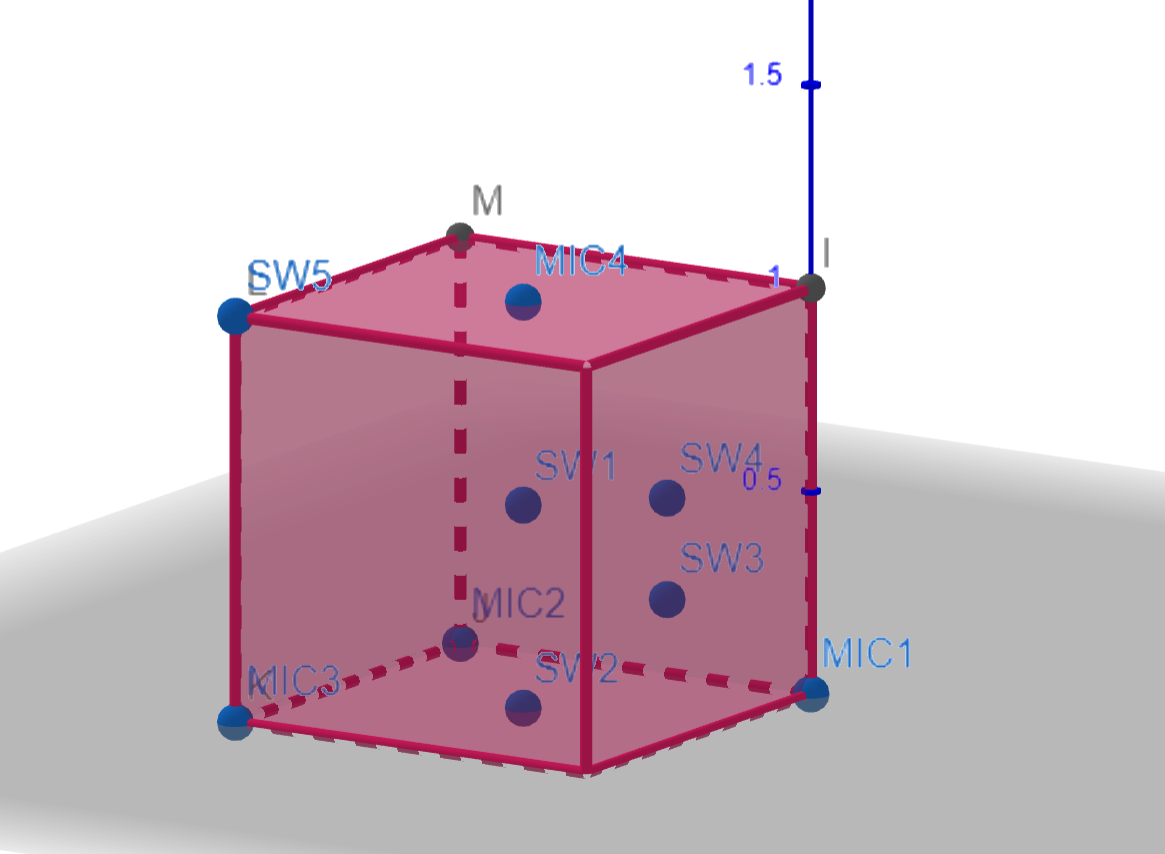
\includegraphics[width=0.4\textwidth]{Lage_MIC_Start_AW1}
\caption{Lage der Startwerte und der Mikrofone im Raum}\label{fig:Lage der Startwerte und der Mikrofone im Raum}
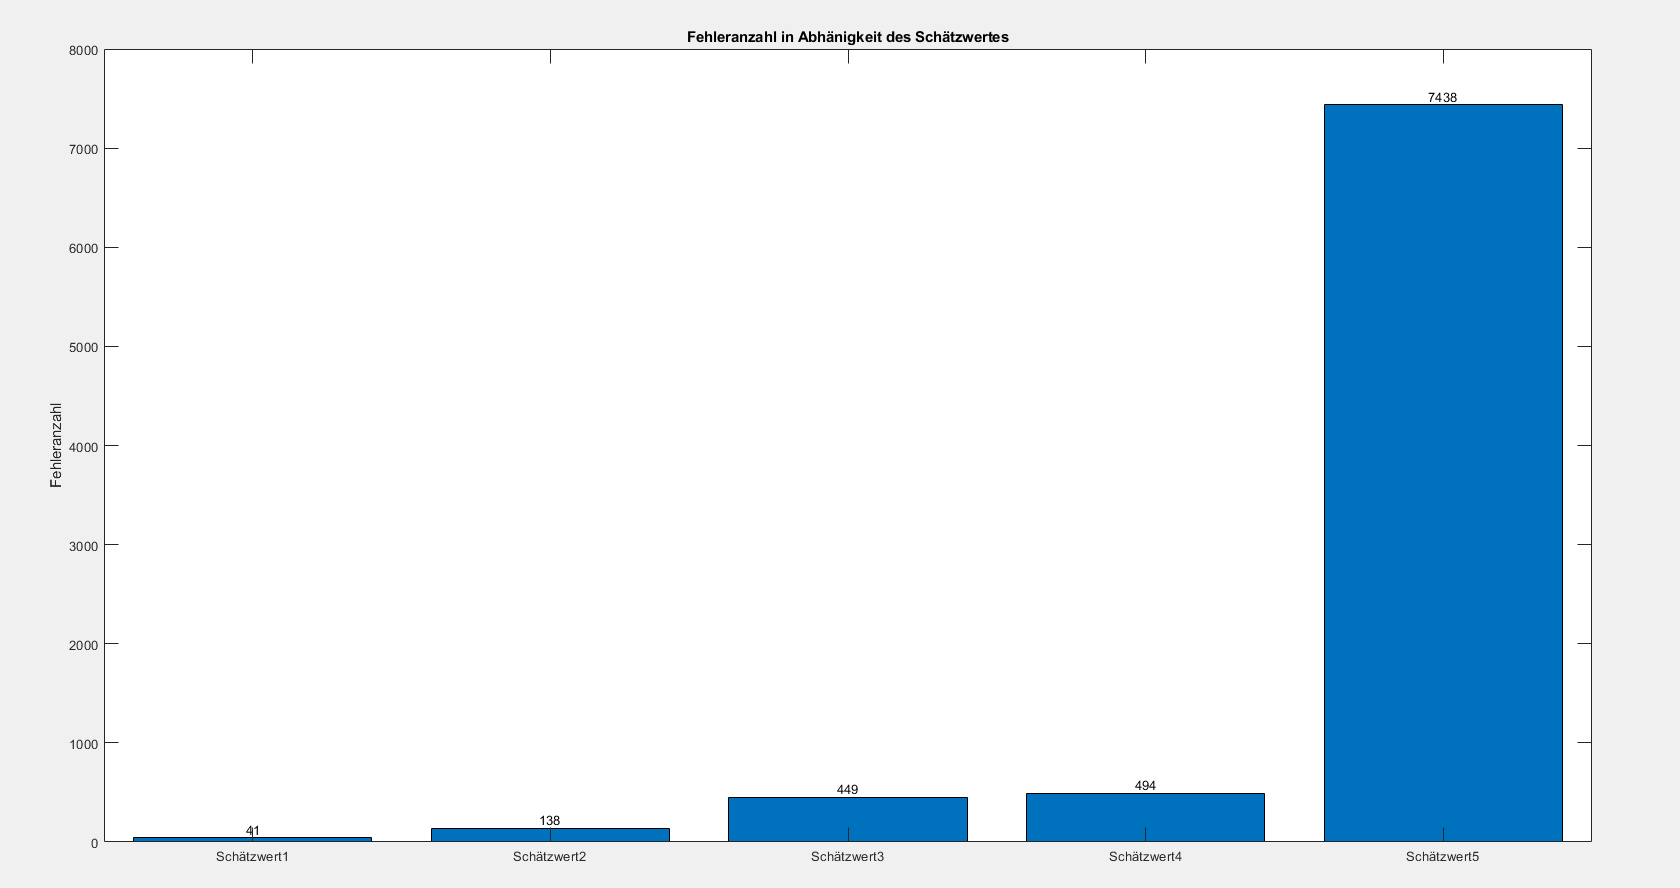
\includegraphics[width=0.4\textwidth]{StartwertZusammenfassung}
\caption{Anzahl der Fehlerfälle mit den einzelnen Startwerten}\label{fig:Anzahl der Fehlerfälle mit den einzelnen Startwerten}
\end{figure}
Die Mikrofone sind annähernd in einen Tetraeder im Raum angeordnet, da dieser die höchste Erfolgsquote bei der Detektion aufweist (siehe "Statistische Auswertung der Fehlerfälle in Abhängigkeit der Positionen der Mikrofone im Raum"). \\
Die fünf Startwerte sind bewusst gewählt, sie stellen besondere Punkte im Raum dar. Startwert 1 ist der Mittelpunkt des Raumes. Startwert 2 stellt den Mittelpunkt der Grundfläche des Raumes dar. Startwert 3 ist der Mittelpunkt eines Quadranten des Raumes. Startwert 4 ist der Mittelpunkt eines Quadranten in x und y Richtung und liegt in der z Richtung exakt auf der Kante der zwei Quadranten. Startwert 5 Stellt einen Eckpunkt des Raumes dar. 
Für das Verständnis der Simulationsbedingungen sind alle relevanten Punkte in der Grafik \ref{fig:Lage der Startwerte und der Mikrofone im Raum} eingezeichnet. \\

Es wurden 10000 mal das Newtonverfahren simuliert. Es wurde für den Ort der Schallquelle jeweils ein Zufallswert innerhalb des Raumes generiert und mit diesem das Verfahren angewendet.
\paragraph{Vermutetes Ergebnis der Simulationen}\ \\
SW 1 sollte die wenigstens Fehler liefern, da der Abstand zum weitest möglich entfernten Punkt im Raum in diesem Fall der Geringste ist. Dadurch müssten möglichst wenige falsche Tangenten durch das Newtonverfahren approximiert werden. Aus dem Umkehrschluss folgt, dass SW 5 das schlechteste Ergebnis liefern müsste, da dort diese Maximaldistanz maximal groß ist. Deshalb sollte das Verfahren dort auch sehr viele Punkte außerhalb des Raumes erreichen und damit Fehler ausgeben.
Die Werte von SW2 SW3 und SW4 liegen dazwischen
\paragraph{Auswertung der Simulationsergebnisse}\ \\
Das Histogramm \ref{fig:Anzahl der Fehlerfälle mit den einzelnen Startwerten} zeigt die Anzahl der fehlerhaften Simulationen von jedem Schätzwert. SW 1 erzeugt 41 Fehler, SW 2 erzeugte 494 Fehler, SW 3 erzeugte 138 Fehler, SW 4 erzeugte 449 Fehler und SW 5 erzeugte 7438 Fehler.
Die Vermutung zum Simulationsergebnis trifft zu. Wobei auffällt,dass der Wert von SW 5 mit 75\% Fehlerquote sehr hoch ist.
Die Fehlerquote bei SW 1 beträgt gerade einmal 0,4 \%  und bei SW 2 bis SW 4 liegt die Quote bei 1\% bis 5\%.
 
\paragraph{Fazit}\ \\
Als Fazit bleibt zu ziehen, dass der Startwert in der Mitte des Raumes die bestmöglichen Ergebnisse liefert. Deswegen ist dieser im Versuchsaufbau zu wählen.


%__________________________________________________________________________________________________
\subsection{Statistische Auswertung der Iterationszahlen des Newtonverfahrens in Abhängigkeit der Raumgröße}
\paragraph{Bedingungen für die Simulation}\ \\
\begin{figure}
\centering 
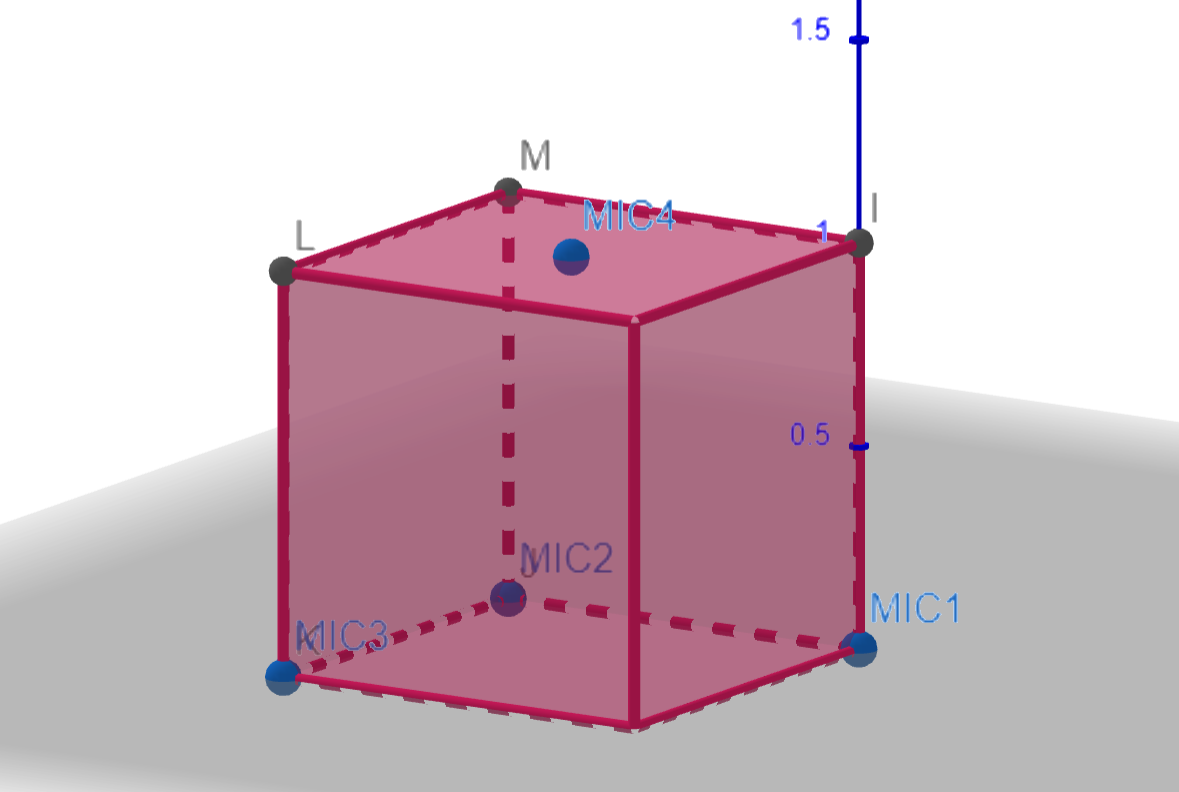
\includegraphics[width=0.4\textwidth]{Lage_MIC_AW2}
\caption{Lage der Mikrophone in einem Raum mit 1 x 1 x 1 m}\label{fig:Lage der Mikrophone in einem Raum mit 1 x 1 x 1 m}
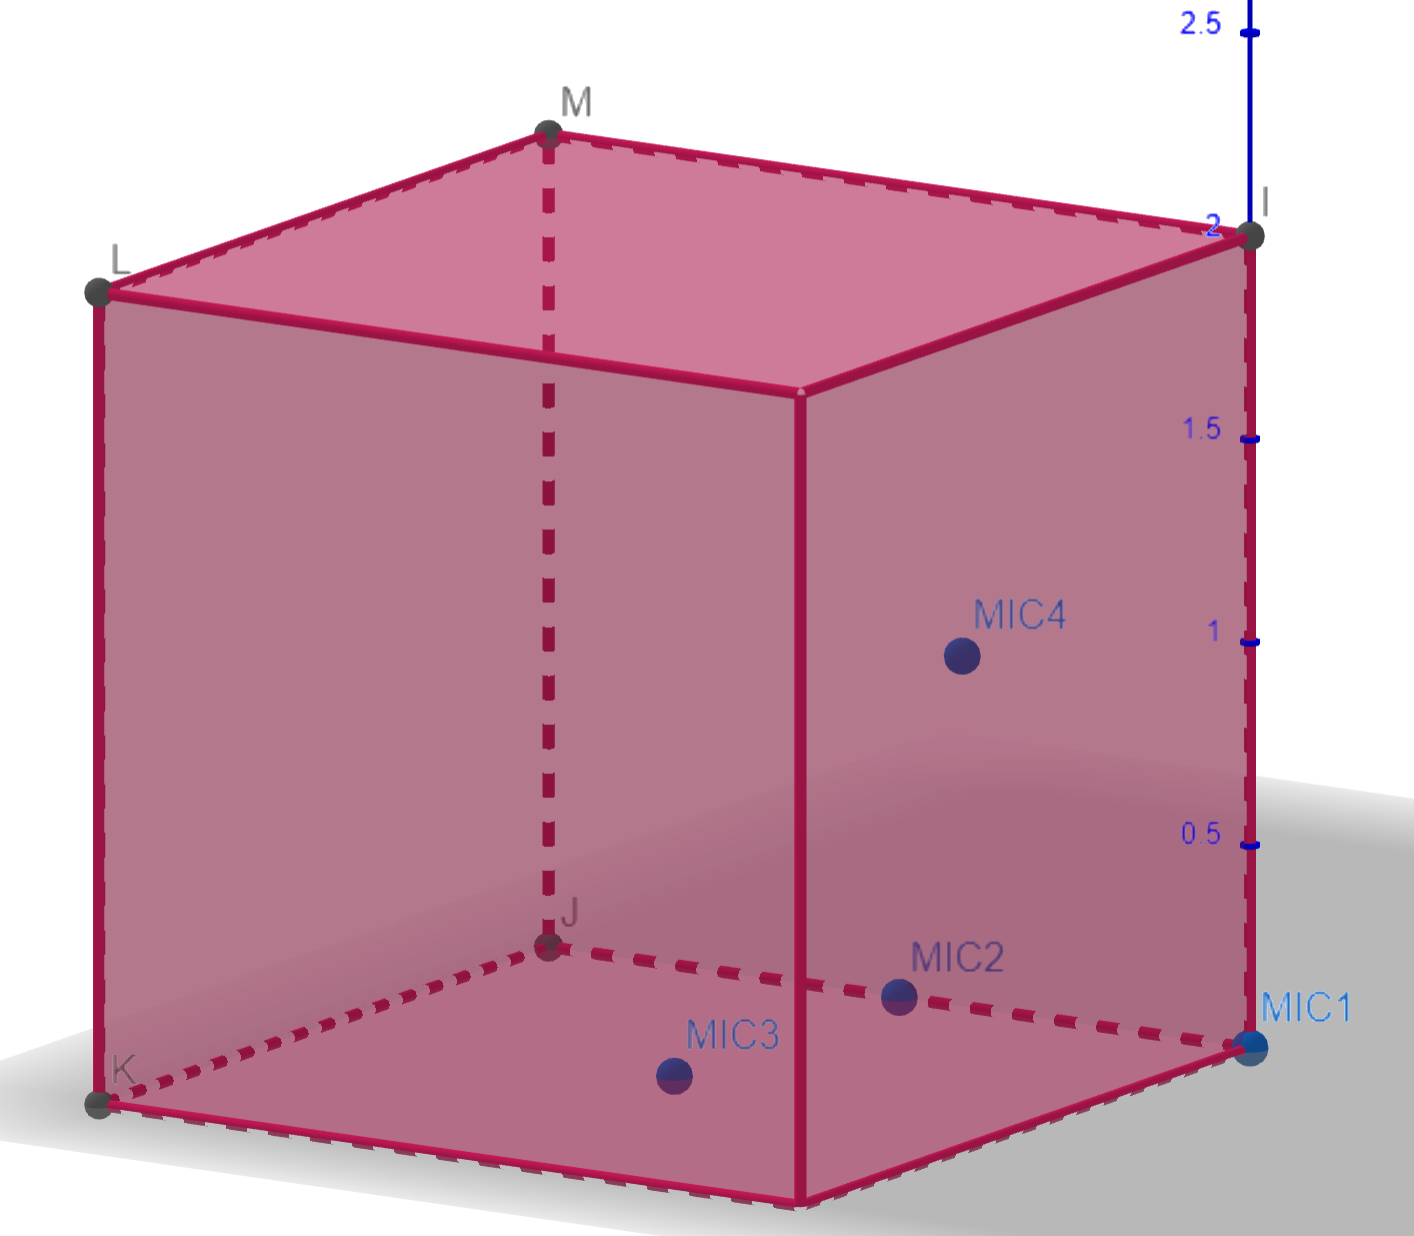
\includegraphics[width=0.4\textwidth]{Lage_MIC_AW2_2}
\caption{Lage der Mikrophone in einem Raum mit 2 x 2 x 2 m}\label{fig:Lage der Mikrophone in einem Raum mit 2 x 2 x 2 m}
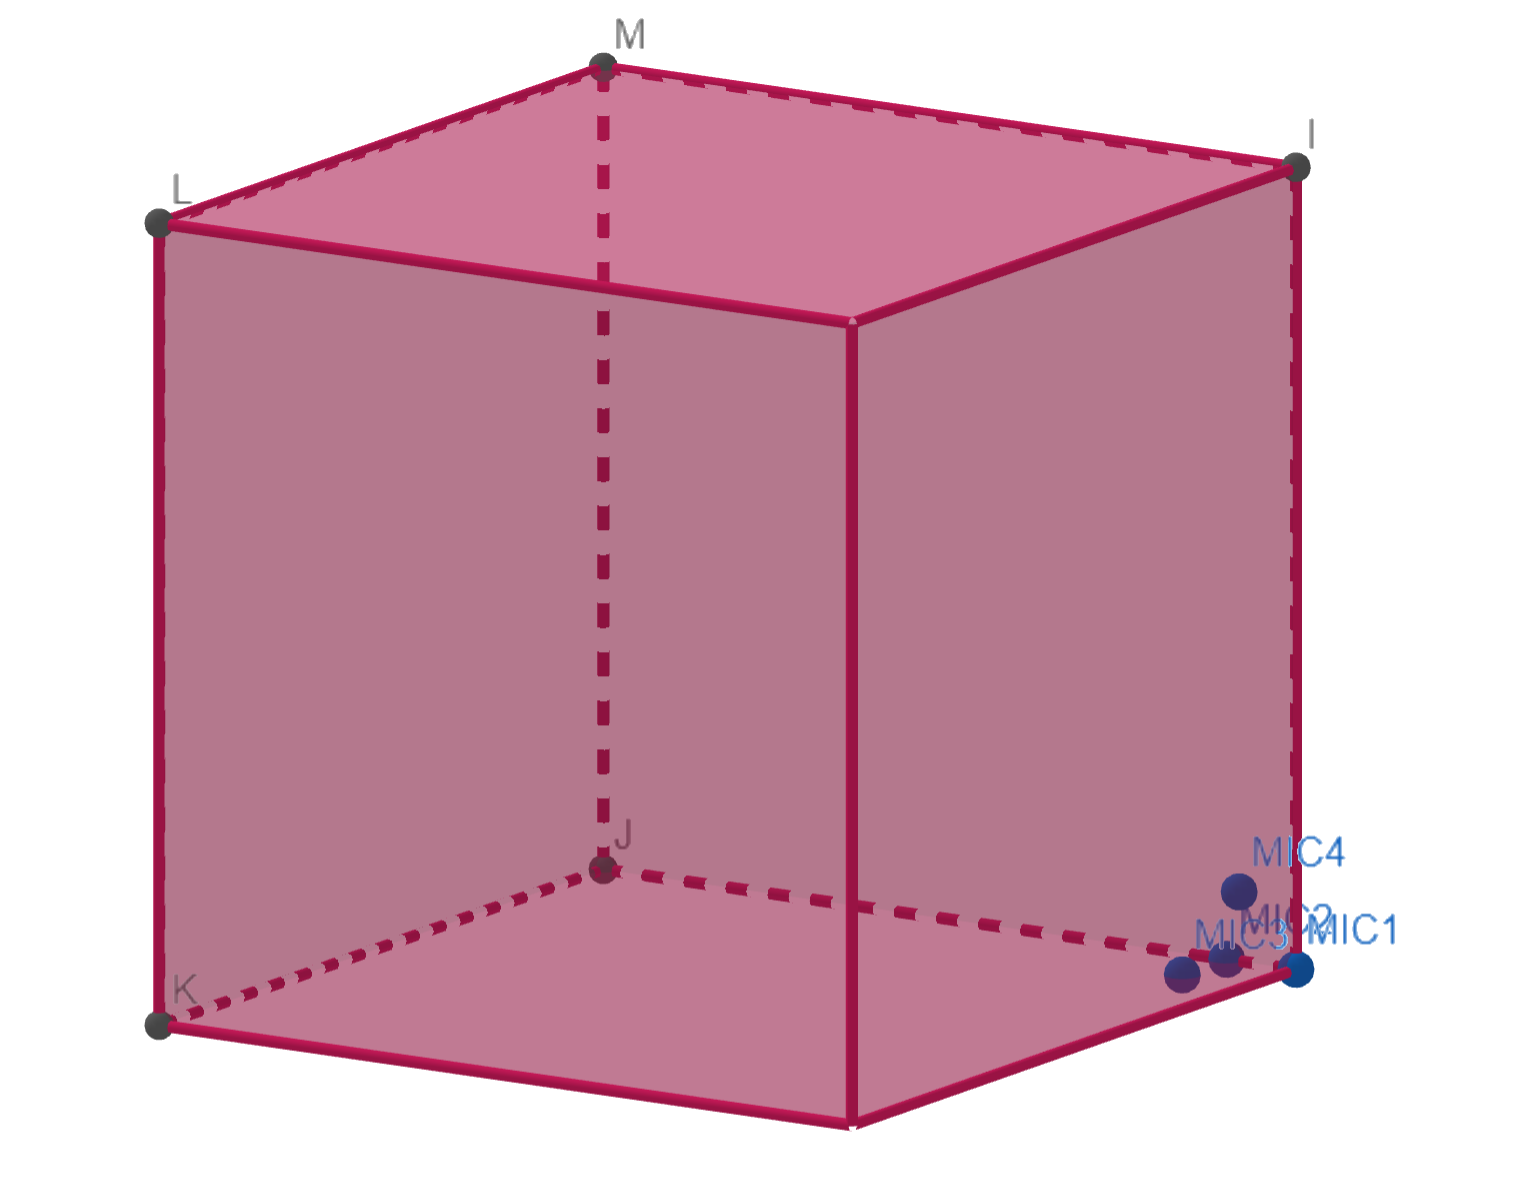
\includegraphics[width=0.4\textwidth]{Lage_MIC_AW2_10}
\caption{Lage der Mikrophone in einem Raum mit 10 x 10 x 10 m}\label{fig:Lage der Mikrophone in einem Raum mit 10 x 10 x 10 m}
\end{figure}
In dieser Simulation wollten wir die Anzahl der benötigten Iterationen herausfinden in Abhängigkeit der Raumgröße. 
Die Positionen der Mikrofone waren immer gleich:\\
MIC1 = (0,0,0)
MIC2 = (1,0,0)\\
MIC3 = (1,1,0)
MIC4 = (0.5,0.5,1)\\

Der Startwert des geschätzten Ortes der Schallquelle blieb ebenfalls gleich: SW1 = (0.5,0.5,0.5)\\

Es wurden wieder 10000 mal für jede Raumgröße simuliert.
Es wurden nur die Simulationen bewertet, in denen das Newtonverfahren zu einem Ergebnis kam. Die Fehlerfälle flossen nicht in die Statistik mit ein.  Zur Visualisierung der Simulationsbedingungen siehe die Grafiken 7, 8 und 9.\\

\paragraph{Vermutetes Ergebnis der Simulationen}\ \\
Mit zunehmender Raumgröße muss die Anzahl der benötigten Iterationen steigen, da nun der mittlere Abstand zwischen geschätztem Ort der Schallquelle und dem realen Ort steigt.
Darüber, ob der Zusammenhang linear oder exponentiell ist, können wir keine Vermutung anstellen.
\paragraph{Auswertung der Simulationsergebnisse}\ \\
\begin{figure}
\centering 
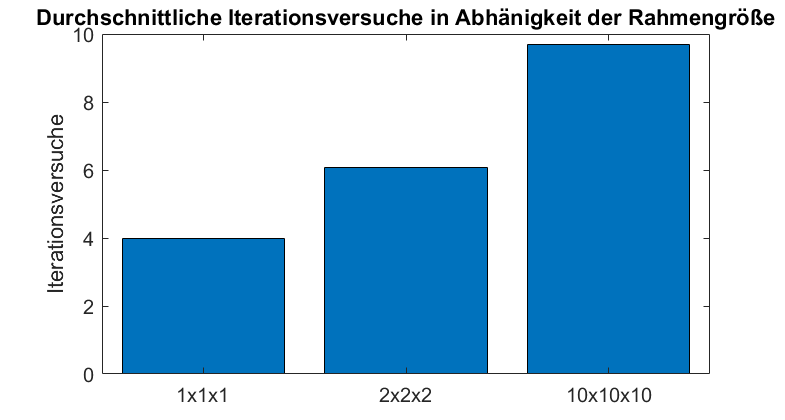
\includegraphics[width=0.4\textwidth]{DurchschnittlicheIterationsversuche}
\caption{Anzahl der Durchschnittlichen Iterationsversuche in Abhängigkeit der Raumgröße in $m^{2}$}\label{fig:Anzahl der Durchschnittlichen Iterationsversuche in Abhängigkeit der Raumgröße in m}
\end{figure}
Die Durchschnittsiterationsanzahl betrug bei 1 $m^{2}$ Raumgröße 4. Bei 8 $m^{2}$ Raumgröße wurden durchschnittlich 6 Iterationen  benötigt um, zum Ort der Schallquelle zu gelangen. Bei 1000 $m^{2}$ wurden im Schnitt 10 Iterationen benötigt. Dies zeigen die Histogramme aus Grafik 10. In diesen sind die Iterationsanzahl über die Raumgröße aufgetragen. \\ Es ist also eindeutig ein Zusammenhang aus steigender Raumgröße und einer Mehrzahl an benötigten Iterationen zu sehen. Dieser ist aber nicht linear, sonder eher sehr schwach exponentiell.
\paragraph{Fazit}\ \\
Die Größe des Raumes und damit der Abstand von geschätztem zu realem Ort der Schallquelle hat nur einen geringen Einfluss auf die benötigte Anzahl an Iterationen. Die Häufigkeit der Fehler aus  der Auswertung des geschätzten Ortes  rührt also nicht aus dem eben beschriebenen, gestiegenen Abstand her, bei der Wahl der verschiedenen Schätzwerte. Es muss daran liegen, dass das Newtonverfahren durch schlechte Schätzwerte dann sich an andere Tangentialebenen annähert, als an die Gesuchte.
%________________________________________________________________________________________________________________
\subsection{Statistische Auswertung der Fehlerfälle in Abhängigkeit der Positionen der Mikrofone im Raum}\label{sec:Position}
\paragraph{Bedingungen für die Simulation}\ \\ 
Die Raumgröße beträgt 1 x 1x 1 m.
Der Startwert für die Schätzung des Ortes der Schallquelle ist für alle Simulationen gleich und hat die Koordinaten (0.5,0.5,0.5). Es wurden für jede Mikrofonpositionierung 1000 Wiederholungen mit jeweils zufällig erzeugtem Ort der Schallquelle durchgeführt. 
Die Mikrofonpositionierungen sind:\\
MP1:\\
MIC1 = (1,0,0)
MIC2 = (1,1,0)\\
MIC3 = (0,1,0)
MIC4 = (0,0,1)\\
MP2:\\
MIC1 = (0.75,0.25,0.25)
MIC2 = (0.75,0.75,0.25)\\
MIC3 = (0.25,0.75,0.25)
MIC4 = (0.25,0.25,0.75)\\
MP3:\\
MIC1 = (0.6,0.4,0.4)
MIC2 = (0.6,0.6,0.4)\\
MIC3 = (0.4,0.6,0.4)
MIC4 = (0.4,0.4,0.6)\\ 
MP4:\\
MIC1 = (0,0,0)
MIC2 = (1,0,0)\\
MIC3 = (0.5,1,0)
MIC4 = (0.25,0.25,0.75)(0.5,0.5,1)\\
MP5:\\
MIC1 = (0,0,0)
MIC2 = (1,0,0)\\
MIC3 = (1,1,0)
MIC4 = (0.5,0.5,1)\\
\begin{figure}
\begin{minipage}[t]{0.33\linewidth}
\centering 
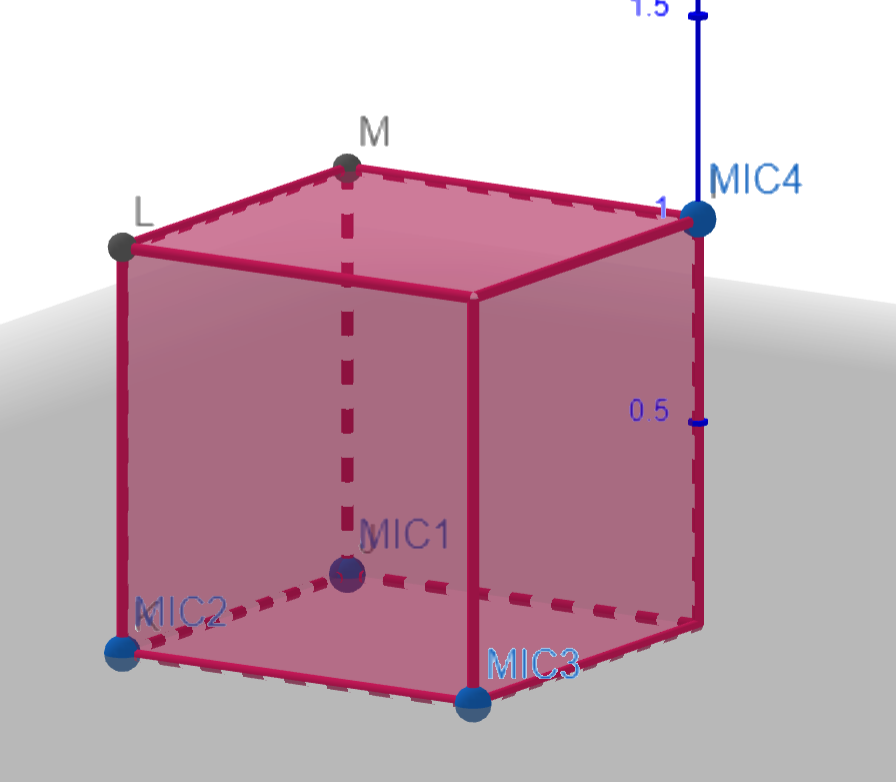
\includegraphics[width=0.4\textwidth]{MP1}
\caption{Lage der Mikrophone in Variante 1}\label{fig:Lage der Mikrophone Variante 1}
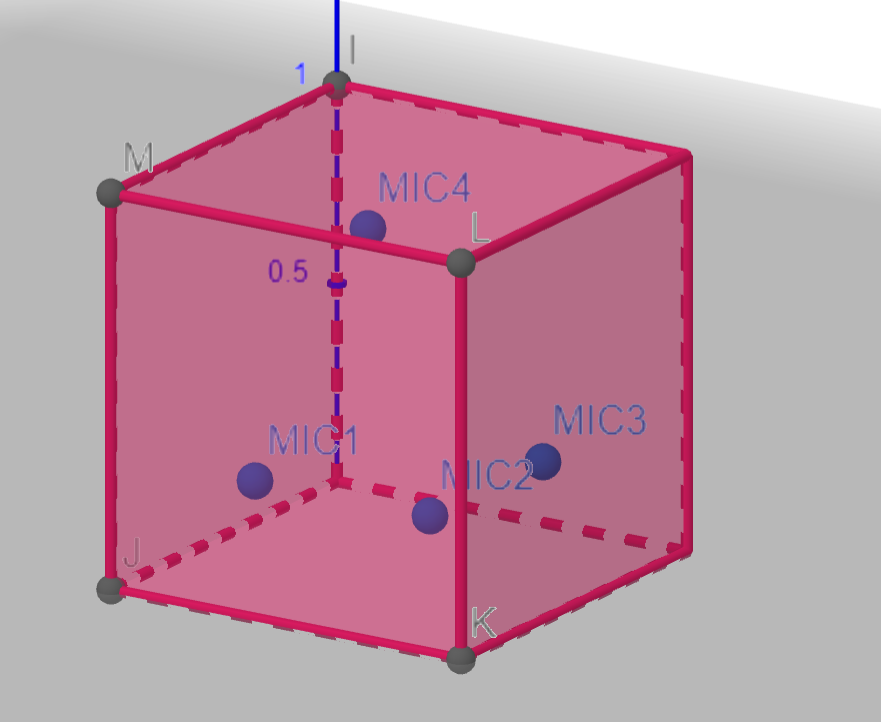
\includegraphics[width=0.4\textwidth]{MP2}
\caption{Lage der Mikrophone in Variante 2}\label{fig:Lage der Mikrophone in Variante 2}
\end{minipage}
\begin{minipage}[t]{0.33\linewidth}
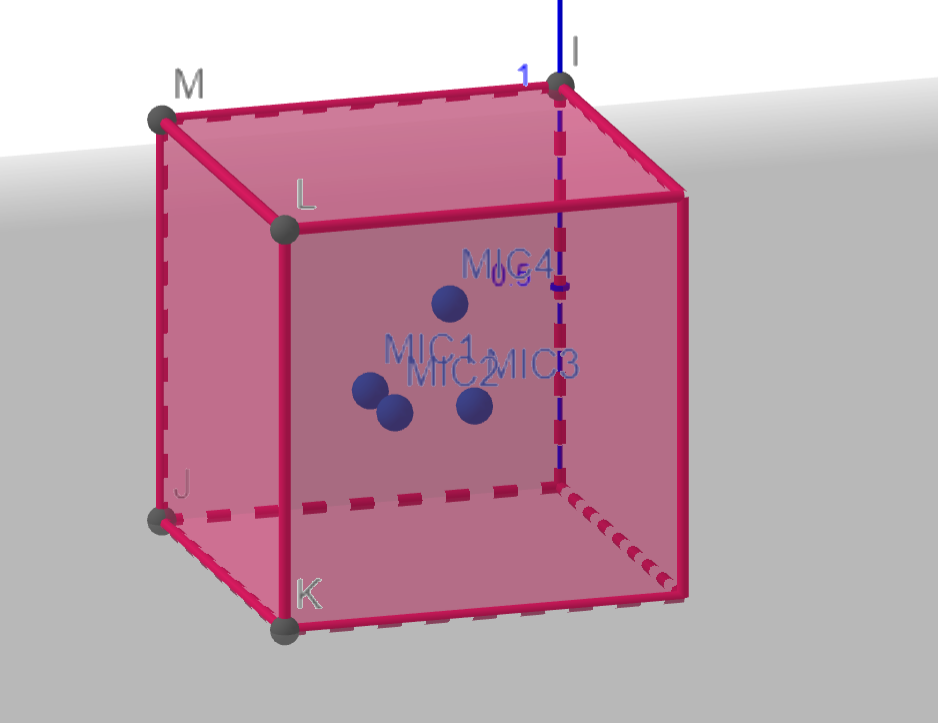
\includegraphics[width=0.4\textwidth]{MP3}
\caption{Lage der Mikrophone in Variante 3}\label{fig:Lage der Mikrophone in Variante 3}
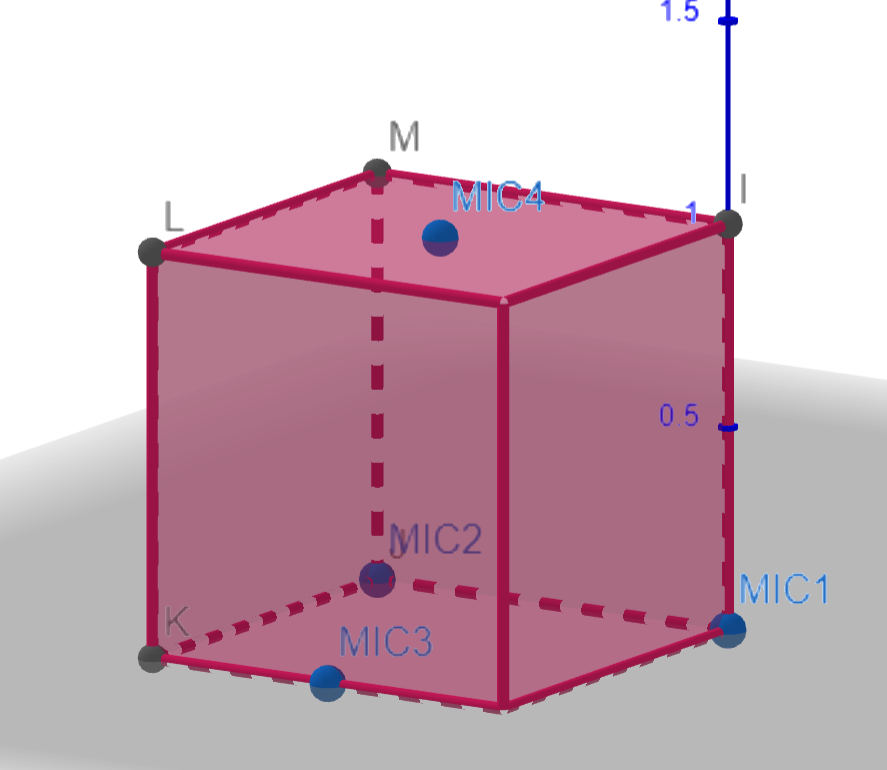
\includegraphics[width=0.4\textwidth]{MP4}
\caption{Lage der Mikrophone in Variante 4}\label{fig:Lage der Mikrophone Variante 4}
\end{minipage}
\begin{minipage}[t]{0.33\linewidth}
\centering
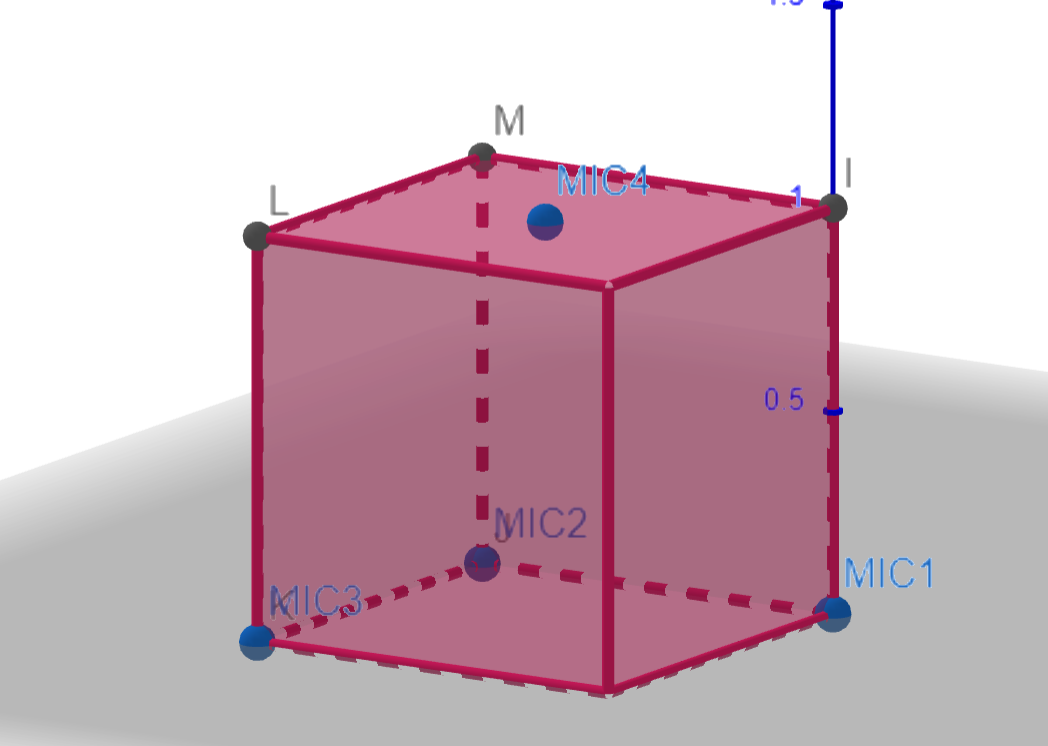
\includegraphics[width=0.4\textwidth]{MP5}
\caption{Lage der Mikrophone in Variante 5}\label{fig:Lage der Mikrophone in Variante 5}
\end{minipage}
\end{figure}
Zur einfacheren Visualisierung sind die Mikrofonkonstellationen in den Grafiken 11 bis 15 dargestellt. \\
In MP1 bilden drei der Mikrofone ein Dreieck in einer Fläche, das vierte Mikrofon befindet sich in einer anderen Höhe, außerhalb der Dreiecksfläche.\\
In MP2 ist die Anordnung nach der selben Grundidee, wie bei MP1. Allerdings sind alle Punkte um den Faktor 0.75 näher an das Zentrum des Raumes verschoben.\\
In MP3 ist es ebenfalls die selbe Anordnung wie bei MP1, hier sind sie aber bis auf den Faktor 0.9 an das Zentrum des Raumes verschoben.\\
In MP4 wird die Grundfläche eines Dreiecks aus Mikrofonen aus einer Kante des Raumes, sowie der Seitenhalbierenden der gegenüberliegenden Kante auf der Grundfläche des Raumes gebildet. Das vierte Mikrofon befindet sich in der Mitte der gegenüberliegenden Seite des Raumes. es wird also beinahe ein Tetraeder aufgespannt. \\
In MP5 ist der Aufbau ähnlich zu MP4. Nur das Mikrofon, das in der Seitenhalbierenden der gegenüberliegenden Kante positioniert war, wird auf eine, der noch freien Ecken der Grundfläche, verschoben. Es ähneln sich also MP1, MP2 und MP3. Sowie MP4 und MP5 weißen Gemeinsamkeiten auf.

\paragraph{Vermutetes Ergebnis der Simulationen}\ \\
Die Anzahl der der Fehler müsste von MP1 bis MP3 zunehmen, da sich die Grundlegende Geometrie nicht ändert, aber der Gangunterschied der Signale an den Mikrofonen immer mehr verringert. Dies resultiert aus dem kleiner werdenden Abstand zwischen den Mikrofonen. Wegen dieser Tatsache müssten auch die Werte von MP5 besser sein, als die von MP4. Da dort die Distanzen zwischen den Mikrofonen größer sind.\\
Ob die Anzahl der  Fehler bei der Geometrie MP1 oder MP5 besser ist, können wir nicht vorhersehen. Dafür müssen die Simulationsergebnisse ausgewertet werden.
\paragraph{Auswertung der Simulationsergebnisse}\ \\
\begin{figure}
\centering 
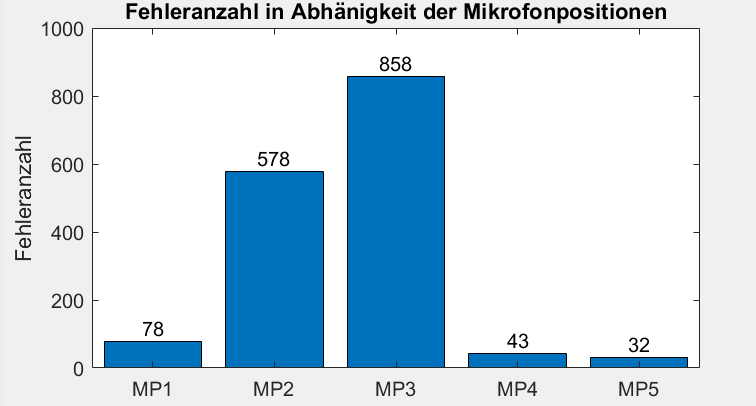
\includegraphics[width=0.4\textwidth]{MikroPositionZusammenfassung}
\caption{Anzahl der Fehler pro 1000 Iterationen bei verschiedenen Mikrofonkonstellationen}\label{fig:Anzahl der Fehler pro 1000 Iterationen bei verschiedenen Mikrofonkonstellationen}
\end{figure}

Im Histogramm Grafik 16 sind die Anzahlen der fehlerhaften Verfahrensdurchläufe über die Mikrofonkonstellationen abgebildet. MP1 erzeugt 78 Fehler. Bei MP2 waren es 578 und bei MP3 858. Bei MP4 wurden 43 Durchläufe Fehlerhaft, bei MP5 waren es 32. MP5 erzeugt somit die wenigsten Fehler und wird deshalb im Aufbau verwendet. Diese Mikrofonkonstellation wurde ebenfalls verwendet, um die anderen Simulationen zu erstellen, da sie die exaktesten Ergebnisse versprach.
\paragraph{Fazit}\ \\
Die Vermutung traf zu, dass mit Verringerung des Abstandes zwischen den Mikrofonen die Fehlerrate stark steigt. Der Effekt ist bei MP1 bis MP3 fast linear. Wenn der Abstand ~ * 0.6 Betrug wuchs die Fehlerzahl um Faktor 6. Bei einem Abstand ~ *0.9 wuchs die Fehleranzahl um Faktor 9. \\
Bei MP4 zu MP5 ist ein Faktor nicht direkt ableitbar, aber die Ergebnisse deuten in die selbe Richtung. Größerer Abstand führt zu besseren Ergebnissen.
Da die Fehleranzahl von MP5 deutlich geringer ist, als die von MP1, scheint die Geometrie mit der "Pyramidenspitze" oberhalb der Grundfläche besser zu sein, als die außerhalb der Grundfläche.
%_________________________________________________________________________________________________________________


\subsection{Evaluierung mit zufälligem Fehler $\pm$ $\varepsilon$}
Ein Fehler bei der Bestimmung der Laufzeitdifferenzen kann durch viele Einflüssen entstehen, wir wollen uns hier auf die zwei signifikantesten fokussieren. Der Fehler soll hier der Abstand der Schallquelle zur Position der berechneten Schallquelle.
\paragraph{Auswirkung der Abtastrate des Mikrocontrollers}
Das analoge Audio-Signal muss in ein digitales Signal umgewandelt werden, um verarbeitet werden zu können. Der A/D Wandler hat jedoch eine endliche Abtastrate. Dies führt zu einem Digitalisierungsfehler. Durch eine Simulation haben wir herausgefunden, wie die Abtastrate mit dem Fehler korreliert. An der Abbildung ist zu erkennen, dass der Fehler proportional zu 1/Abtastrate ist. Ein Raspberrry Pi hat zum Beispiel eine Abtastrate von 100kSamples pro Sekunde. Bei dieser Abtastrate, entsteht ein Fehler von durchschnittlich 2,5 mm.

\paragraph{Auswirkung der Schallgeschwindigkeit}
Bei unseren Berechnungen sind wir bis jetzt immer von der Schallgeschwindigkeit von 343 m/s ausgegangen. Dies ist die Standard Geschwindigkeit bei 20° Celsius Lufttemperatur. Die Schallgeschwindigkeit ist proportional zu $\sqrt{\vartheta}$. Wenn also die Temperatur schwankt, beeinflusst dies auch die Schallgeschwindigkeit. 
\begin{align}
c\vartheta = c0 * \sqrt{1+\alpha * \vartheta}\\   
c\vartheta =  331,4 m/s * \sqrt{1 + 1/273,15 * \vartheta}
\end{align}
Dies führt zu Fehlern in den Laufzeitdifferenzen, die unsere Mikrofone aufnehmen. Eine Temperaturdifferenz der angenommenen Temperatur zur wahren Temperatur hat verfälscht also die Berechnete Position der Schallquelle. Dies haben wir mit MATLAB simuliert. In der Abbildung ist zu erkennen, dass der Fehler proportional zur Temperaturdifferenz ist. Wenn wir also mit unserer angenommen Temperatur um 20° Celsius daneben liegen, dann wird der Laser das Ziel um 30 mm verfehlen. Dieser Fehler ist besonders fatal, da es sich hierbei um einen systematischen Fehler handelt. Wir müssen also die schwankende Schallgeschwindigkeit kompensieren, um unser Ziel zu treffen.

\begin{figure}
\centering 
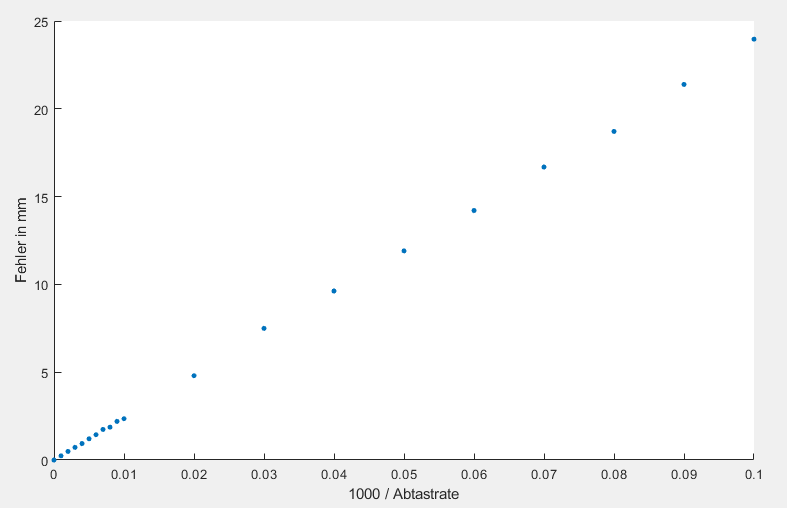
\includegraphics[width=0.4\textwidth]{Chart Abtastrate}
\caption{Einfluss der Abtastrate auf die Genauigkeit der Positionsbestimmung}\label{fig:Einfluss der Abtastrate auf die Genauigkeit der Positionsbestimmung}
\end{figure}

\begin{figure}
\centering 
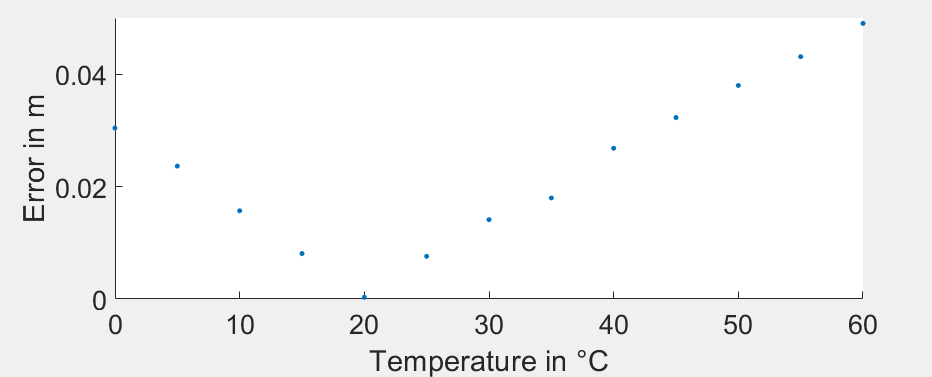
\includegraphics[width=0.4\textwidth]{Chart Temperatur}
\caption{Einfluss der Temperatur auf die Genauigkeit der Positionsbestimmung}\label{fig:Einfluss der Temperatur auf die Genauigkeit der Positionsbestimmung}
\end{figure}
%_________________________________________________________________________________________________
\subsection{Auswahl der bestmöglichen Parametrierung unter Berücksichtigung der Ergebnisse der Analysen}
Nach Abschluss aller Simulationen bleibt als Fazit zu ziehen, dass als Abbruchbedingung für das Newtonverfahren eine Annäherung auf $<$ 1mm zu genau ist, da in der Realität die Störfaktoren durch den Linearisierungsfehler, sowie die veränderte Schallgeschwindigkeit im Extremfall eine Abweichung von $>$ 30mm darstellen.\\
Als geschätzter Startwert sollte der Mittelpunkt des Raumes gewählt werden und die Mikrofone sollten möglichst mit größtmöglichen Abstand, in einer tetraedrischen Anordnung, im Raum verteilt werden. Im vorliegenden Fall bedeutet dies einen Startwert von SW = (0.5,0.5,0.5) und eine Mikrofonpositionierung an den Orten: \\
MIC1 = (0,0,0)
MIC2 = (1,0,0)\\
MIC3 = (1,1,0)
MIC4 = (0.5,0.5,1).